\section{Modello di sviluppo}
Il modello di sviluppo adottato dal gruppo è il \textbf{modello incrementale}.
\subsection{Modello incrementale}
Il modello di sviluppo incrementale vede il progetto come una serie di rilasci (interni e/o esterni), cosiché ad ogni scadenza, il materiale consegnato sia sempre più vicino al prodotto finale.
Questo approccio di sviluppo, vede la specifica del software, la sua implementazione, convalida ed evoluzione, come attività intrecciate tra loro e da sviluppare in parallelo. Quindi il prodotto è considerato tale solo all'ultimo rilascio. Motivo per cui, si relaziona bene con il versinamento adottato per il sistema.
L'adozione dello sviluppo incrementale porta i seguti vantaggi:
\begin{itemize}
\item costi ridotti di implementazione;
\item facilità nell'ottenere feedback;
\item possibilità di consegnare prototipi.
\end{itemize}
Svantaggi del modello incrementale:
\begin{itemize}
\item il processo non è visibile, e il manager deve richiedere consegne frequenti e regolari;
\item inclinazione alla degradazione del sistema, ovvero, la difficoltà di aggiungere funzionalità al sistema in un rilascio successivo, dopo averne integrata un'altra nella consegna attuale. È possibile rimediare tramite refactoring.
\end{itemize}
\begin{figure}[H]
	\centering
	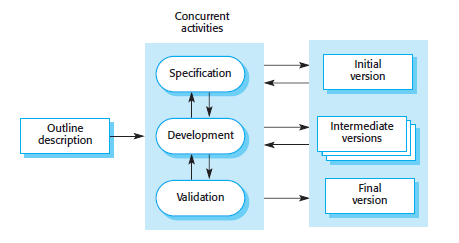
\includegraphics[width=0.70\linewidth]{img/incremental_development.png}
	\caption{Modello di sviluppo incrementale}
\end{figure}